\documentclass[../main.tex]{subfiles}

\graphicspath{{\subfix{../images/}}}

\begin{document}

\section{Part 2 - Measurements}

\subsection{Task 1: VCC/GND bounce 1 output}

Remove jumpers

\begin{itemize}
    \item J1: Output 1Y1-4 enable (QFN)
    \item J4: Output 1y1-4 enable (SOIC)
    \item J9: CLK fanout 1G enable
\end{itemize}

Consult the circuit diagram. Which channel (output) is now active on Driver QFN and Driver SOIC? Connect probe 2 to the active output probe point, and confirm the waveform is as expected. Use probe 2 as a trigger signal.

\vspace{10pt}

Confirm that jumper J3: bounce sense to GND (QFN) is in place. Connect probe 1 to P39: VCC/GND bounce (QFN) and measure the ground bounce.

\solution

The measurement of the ground and VCC bounce for the QFN- and SOIC packages with one (\textit{1}) active output is shown in Figure \ref{fig:gnd_vcc_output_1}. The results are summarized in Table \ref{tab:output_1}.

\begin{figure}[h]
    \centering
    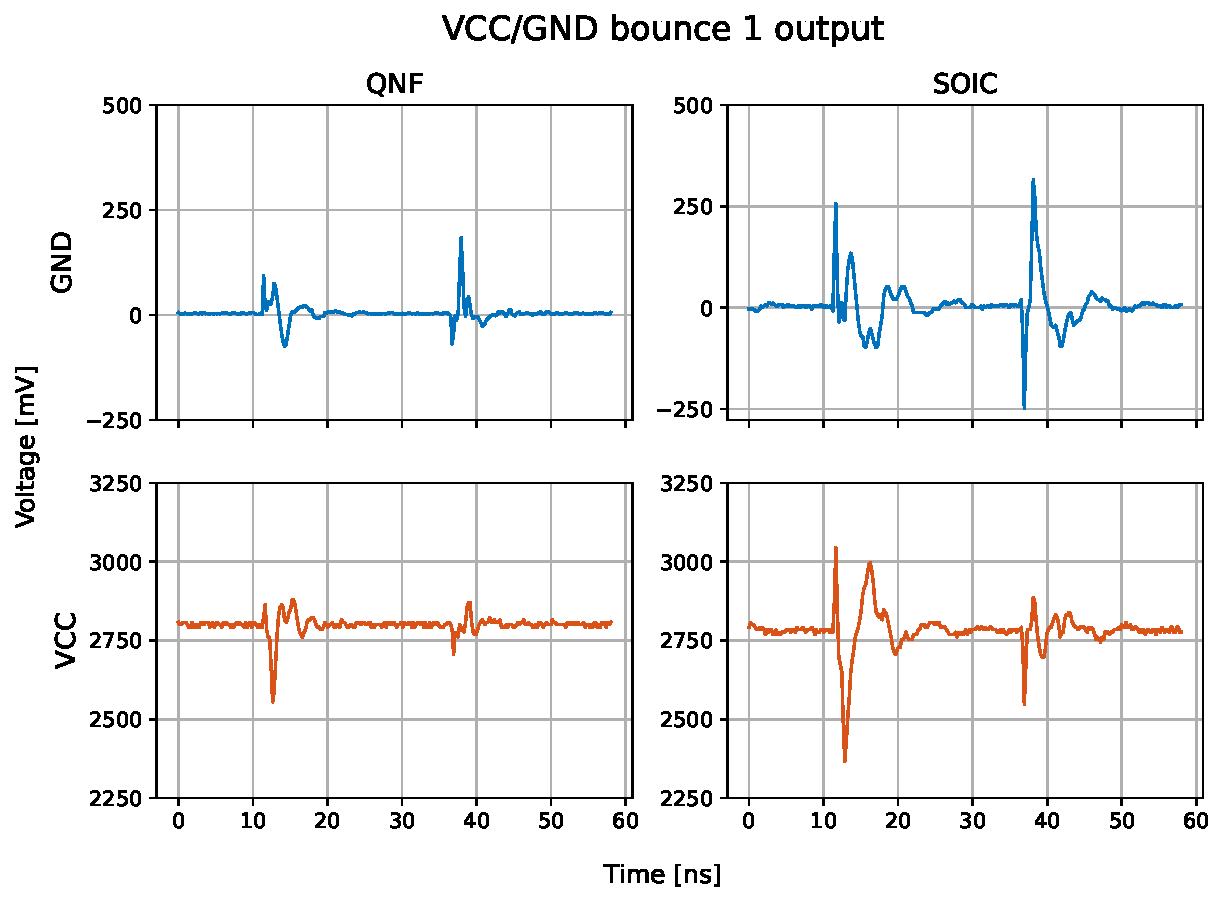
\includegraphics[width=0.8\textwidth]{output_1.pdf}
    \caption{GND and VCC bounce for QFN- and SOIC packages with one (\textit{1}) active output.}
    \label{fig:gnd_vcc_output_1}
\end{figure}

\begin{table}[h]
    \centering
    \begin{tabular}{l | r r}
        \toprule[1pt]
        Package type    & GND [mV]  & VCC [mV]\\
        \midrule
        QFN             & 184.427   & 2547.035  \\
        SOIC            & 324.111   & 2365.217  \\
        \bottomrule[1pt]
    \end{tabular}
    \caption{GND and VCC bounce for QFN and SOIC packages with one (\textit{1}) active output.}
    \label{tab:output_1}
\end{table}

To see whether or not these values are acceptable, we need to compare them to the minimum and maximum allowed values, which can be found in the datasheet for the chip (SN74ALVC244). The data sheets states that, given a supply voltage $V_{CC}$ between 2.7 V and 3.6 V, the 'High-level input voltage', $V_{IH}$ must be at least 2 V. Likewise it states that the 'Low-level input voltage', $V_{IL}$ must be a maximum of 0.8 V. 

However, these are the absolute threshold values, and it might also be useful to look at the noise margins since not all chips are created equal and some might less perfect output. The noise margins are the worst case scenarios and should work for all chips. The noise margins are calculate as follows:

\begin{equation*}
    NM_{L} = V_{IL} - V_{OL} = 0.8 - 0.2 = 0.6 V
\end{equation*}

\begin{equation*}
    NM_{H} = V_{OH} - V_{IH} = (V_{CC} - 0.2) - 2 = 3.3 - 2.2 = 1.1 V
\end{equation*}

Meaning that the GND bounce should ideally be no higher than 0.6 V and the VCC bounce should ideally be no lower than 2.2 V, beyond these values chip is not guaranteed to work as intended as the signals might cross into the undefined region between the high and low logic levels.

\vspace{10pt}

With that mentioned we can now start comparing the results we've gotten from the measurements. Both packages don't have a GND bounce higher than 0.6 V or a VCC bounce lower than 2.2 V, which means that the results are within the acceptable range for both the GND and VCC bounce. All the values are also a good bit from the thresholds, with the closest being the SOIC package's VCC bounce of 2365.217 mV, leaving a 135.217 mV margin for other noise sources to affect the signal before it crosses the threshold.

\subsection{Task 2: VCC/GND bounce 3 outputs}

Place jumper J1 ("Output 1y1-4 enable (QFN)"), J4 ("Output 1y1-4 enable (SOIC)"). Ensure J9 ("CLK fanout 1G enable") is removed, and that J8("CLK fanout 2G enable") is in place.

\vspace{10pt}

Consult the circuit diagram - which channel (output) is now active on Driver QFN and Driver SOIC? Connect probe 2 to the active output probe point, and confirm the waveform is as expected. Use probe 2 as a trigger signal.

\vspace{10pt}

Confirm that jumper J3("Bounce sense to GND(QFN)") is in place. Connect probe 1 to P39("VCC/GND bounce QFN") and measure the ground bounce:

\solution

The measurement of the ground and VCC bounce for the QFN- and SOIC packages with three (\textit{3}) active output is shown in Figure \ref{fig:gnd_vcc_output_3}. The results are summarized in Table \ref{tab:output_3}.

\begin{table}[h]
    \centering
    \begin{tabular}{l | r r}
        \toprule[1pt]
        Package type    & GND [mV]  & VCC [mV]\\
        \midrule
        QFN             & 311.822   & 2301.976  \\
        SOIC            & 515.020   & 2041.107  \\
        \bottomrule[1pt]
    \end{tabular}
    \caption{GND and VCC bounce for QFN and SOIC packages with three (\textit{3}) active outputs.}
    \label{tab:output_3}
\end{table}

To evaluate the results, we again compare them to the minimum and maximum allowed values of 0.6 V and 2.2 V respectively. The QFN package stays within both thresholds but leaves only a margin of 101.976 mV for the VCC bounce, which is acceptable but close to being critical and could prove problematic in high-noise environments. The SOIC package however crosses the VCC bounce threshold with a bounce of 2041.107 mV. This however is still within the absolute thresholds of $V_IH$, leaving the chip operating at the edge of the noise margin, making functionality unreliable in high-noise environments and highly dependent on the individual chips output characteristics.

\newpage

\begin{figure}[h]
    \centering
    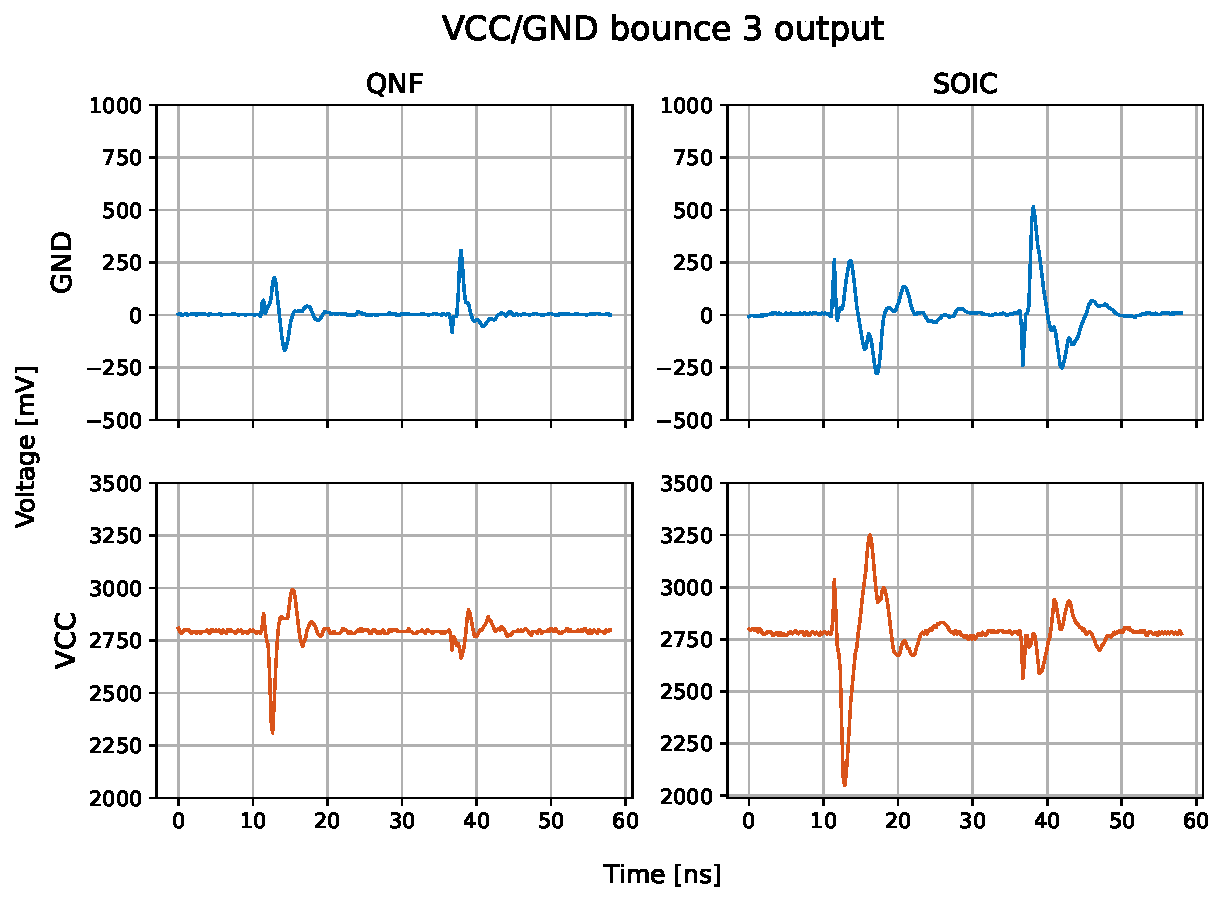
\includegraphics[width=0.8\textwidth]{output_3.pdf}
    \caption{GND and VCC bounce for QFN- and SOIC packages with three (\textit{3}) active output.}
    \label{fig:gnd_vcc_output_3}
\end{figure}

\subsection{Task 3: VCC/GND bounce 7 outputs}

Place all the jumpers on the left. Confirm from the schematic, that all outputs should be enabled. Connect probe 2 to the active output probe point, and confirm the waveform is as expected. Use probe 2 as a trigger signal.

\vspace{10pt}
Confirm that jumper J3("Bounce sense to GND(QFN)") is in place. Connect probe 1 to P39("VCC/GND bounce QFN") and measure the ground bounce:

\solution

The measurement of the ground and VCC bounce for the QFN- and SOIC packages with seven (\textit{7}) active output is shown in Figure \ref{fig:gnd_vcc_output_7}. The results are summarized in Table \ref{tab:output_7}. Once again, the results are compared to the minimum and maximum allowed values. Both packages have VCC bounces that cross both the absolute thresholds. This means that neither package should be used with 7 active outputs, as the bounces are too high crossing the thresholds on their own.

\begin{table}[h]
    \centering
    \begin{tabular}{l | r r}
        \toprule[1pt]
        Package type    & GND [mV]  & VCC [mV]\\
        \midrule
        QFN             & 446.640   & 1983.399  \\
        SOIC            & 782.609   & 1644.712  \\
        \bottomrule[1pt]
    \end{tabular}
    \caption{GND and VCC bounce for QFN and SOIC packages with seven (\textit{7}) active outputs.}
    \label{tab:output_7}
\end{table}

\newpage

\begin{figure}[h]
    \centering
    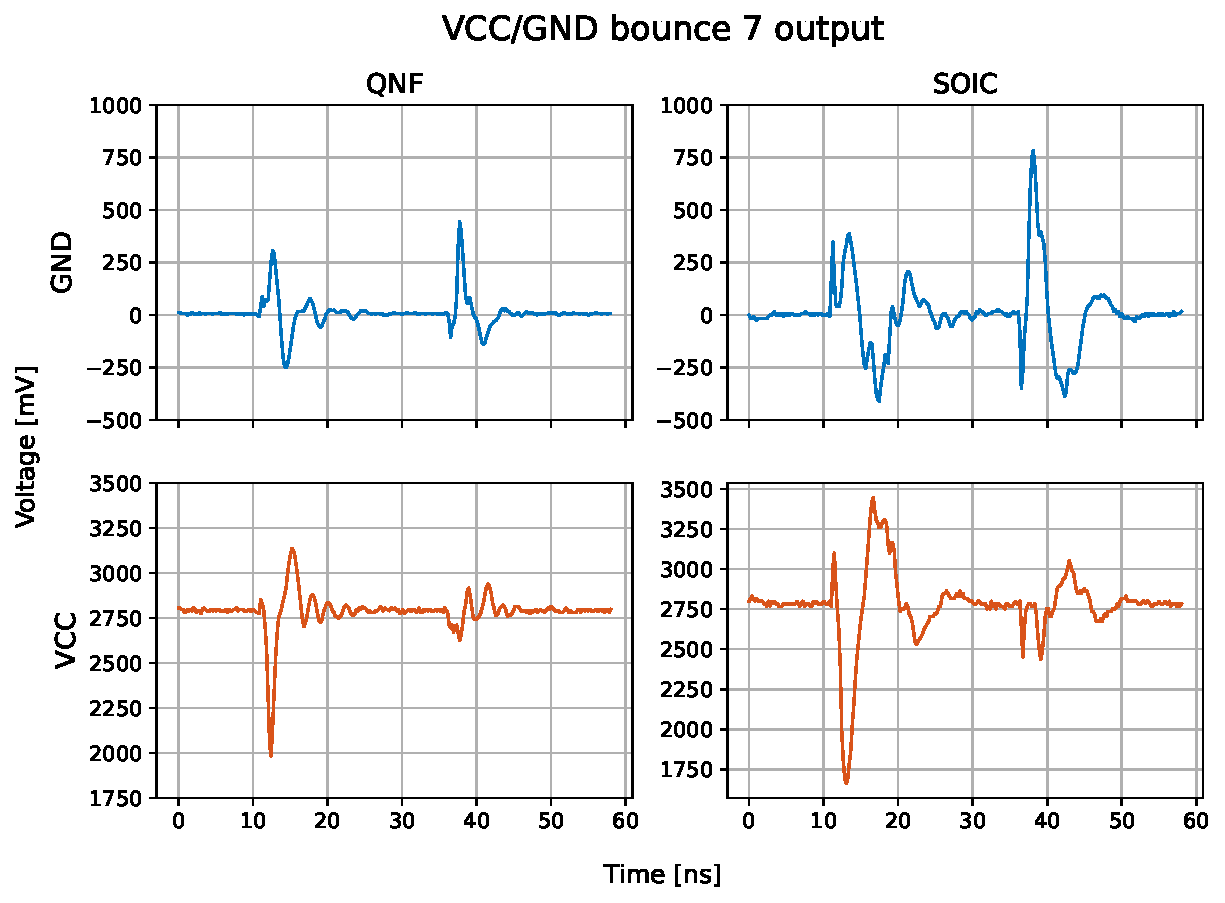
\includegraphics[width=0.8\textwidth]{output_7.pdf}
    \caption{GND and VCC bounce for QFN- and SOIC packages with seven (\textit{7}) active output.}
    \label{fig:gnd_vcc_output_7}
\end{figure}

\subsection{Conclusion on VCC/GND bounce}

\solution

Generally speaking, the QFN package performs better than the SOIC package in regards to VCC and GND bounce. Across the configurations the SOIC package has higher bounces than the QFN package, averaging 72.04\% more on the GND bounce and 25.34\% more on the VCC bounce, relative to an ideal supply voltage of 3.3 V. 

None of the packages should be used with 7 outputs enabled, as the bounces are too high crossing thresholds on their own, risking the chip not functioning properly. 

The QFN package should be able to handle 3 outputs with about 100 mV of leeway before hitting the thresholds, but the SOIC package should not be used with 3 output enabled, since the VCC bounce is high enough to cross the threshold if the individual chip $V_{OH}$ is anything but perfect. For one active output, both packages operate within acceptable thresholds for $V_{IH}$ and $V_{IL}$. 


\newpage

\subsection{Comparison Between Simumlation and Measurement Results}

Also, a section where the measurement results versus the simulations results are compared and discussed, including a discussion/analysis of potential reasons for mismatches (circuit models mismatches, accuracy of measurements, etc.)

\solution

As seen in Figures \ref{fig:sim_v_meas} and \ref{fig:soic-sim_v_meas}, the simulation results are quite far off from the measured results. While they surely give an indication of how the signal can be expected to look, the magnitudes are far off making it hard to estimate real world signal integrity.

\begin{figure}[h]
    \centering
    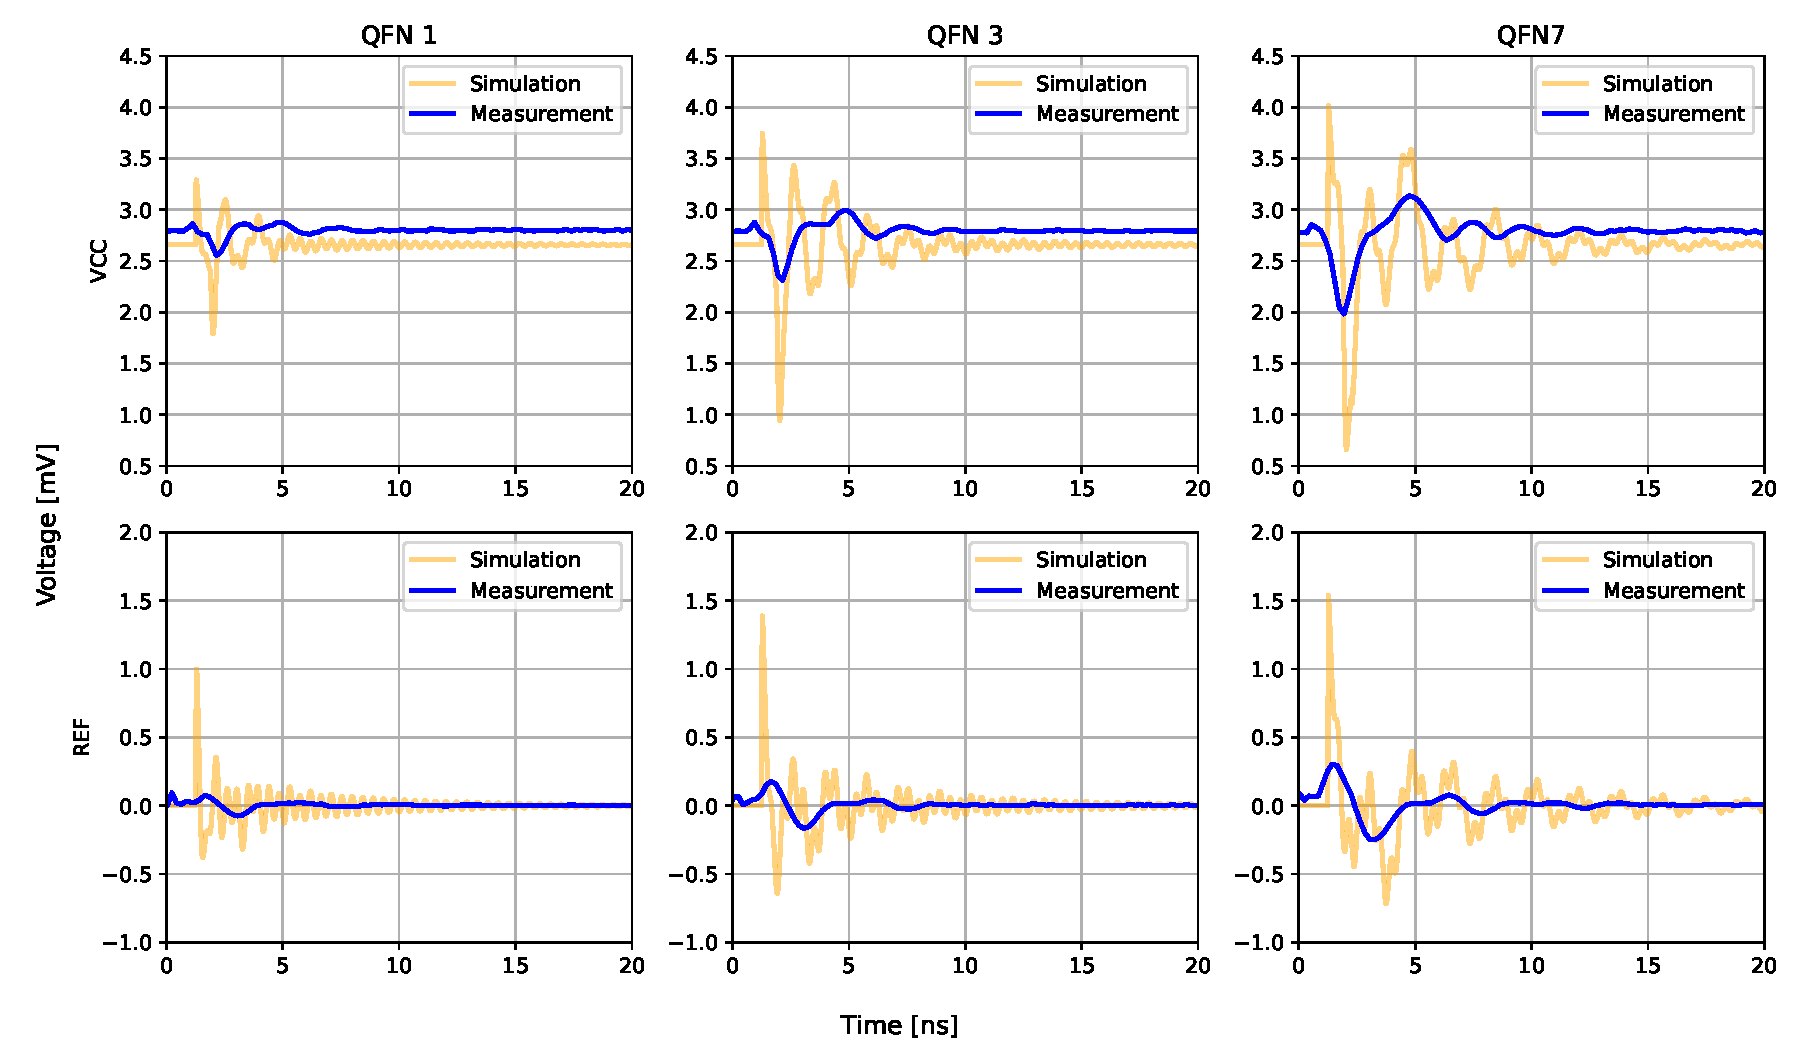
\includegraphics[width=0.8\textwidth]{sim_v_meas.pdf}
    \caption{Comparison between simulation and measurement results for GND and VCC bounce (QFN).}
    \label{fig:sim_v_meas}
\end{figure}

\begin{figure}[h]
    \centering
    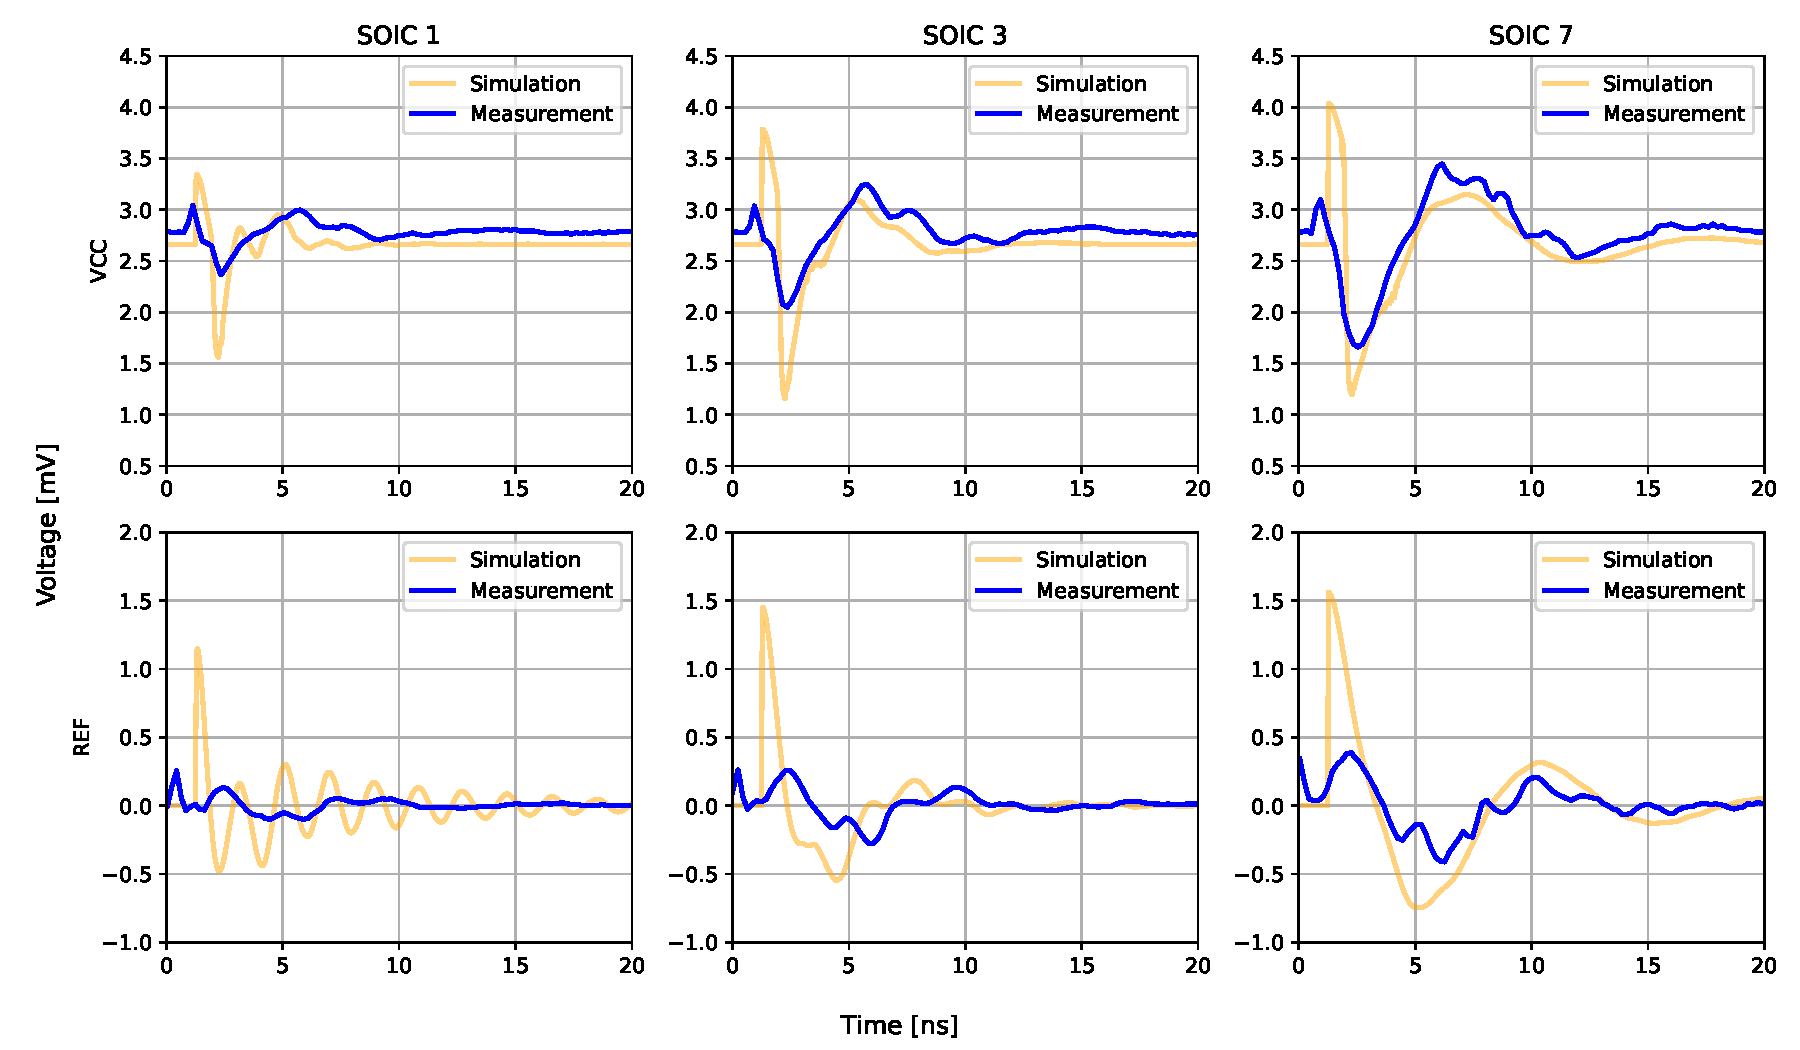
\includegraphics[width=0.8\textwidth]{soic_sim_v_meas.pdf}
    \caption{Comparison between simulation and measurement results for GND and VCC bounce (SOIC).}
    \label{fig:soic-sim_v_meas}
\end{figure}

\newpage

\subsection{Task 4: Inverter GND bounce self-oscillation}

Q5 is a hex inverter, SN74ALVC04. The input is a DC voltage set by a potentiometer marked "Inverter VDC input 0-VCC".

\vspace{10pt}

Confirm that jumper J10 is removed. Only one output on the inverter is active - vary the input using the potentiometer. Can you get the inverter output to oscillate?

\vspace{10pt}

Place jumper J10. All inverter outputs are active - vary the input using the potentiometer. Can you get the inverter output to oscillate? If so, why does it oscillate?

\solution

It was possible to get the inverter output to oscillate when both one and all outputs were active. The oscillations are shown in Figure \ref{fig:inverter_oscillation}. The only noticable differences between the two situations are the amplitude and frequency of the oscillations.

The oscillation occurs because the inverter can act as a feedback system. When the input voltage, controlled by the potentiometer, is near the inverter's switching threshold, $V_{IH}$ or $V_{IL}$, small disturbances or noise, such as GND bounce, at the input can push the input into the undefiend area and cause the inverter to interpret it as the other logic value, cause a switch. This toggling can become self-sustaining, causing the inverter output to oscillate, as the output is fed back into the input, causing the input to switch back and forth between the two logic levels. In effect, this causes the inverter circuit to behave similarly to a ring oscillator. The difference in frequency and amplitude between the two situations can be explained by the number of outputs active. With all outputs active, the bounce is higher, causing the signal to cross the threshold quicker leading to a higher frequency. The amplitude is also higher, as the bounce is higher, causing the signal to cross the threshold with a higher amplitude.

\begin{figure}[h]
    \centering
    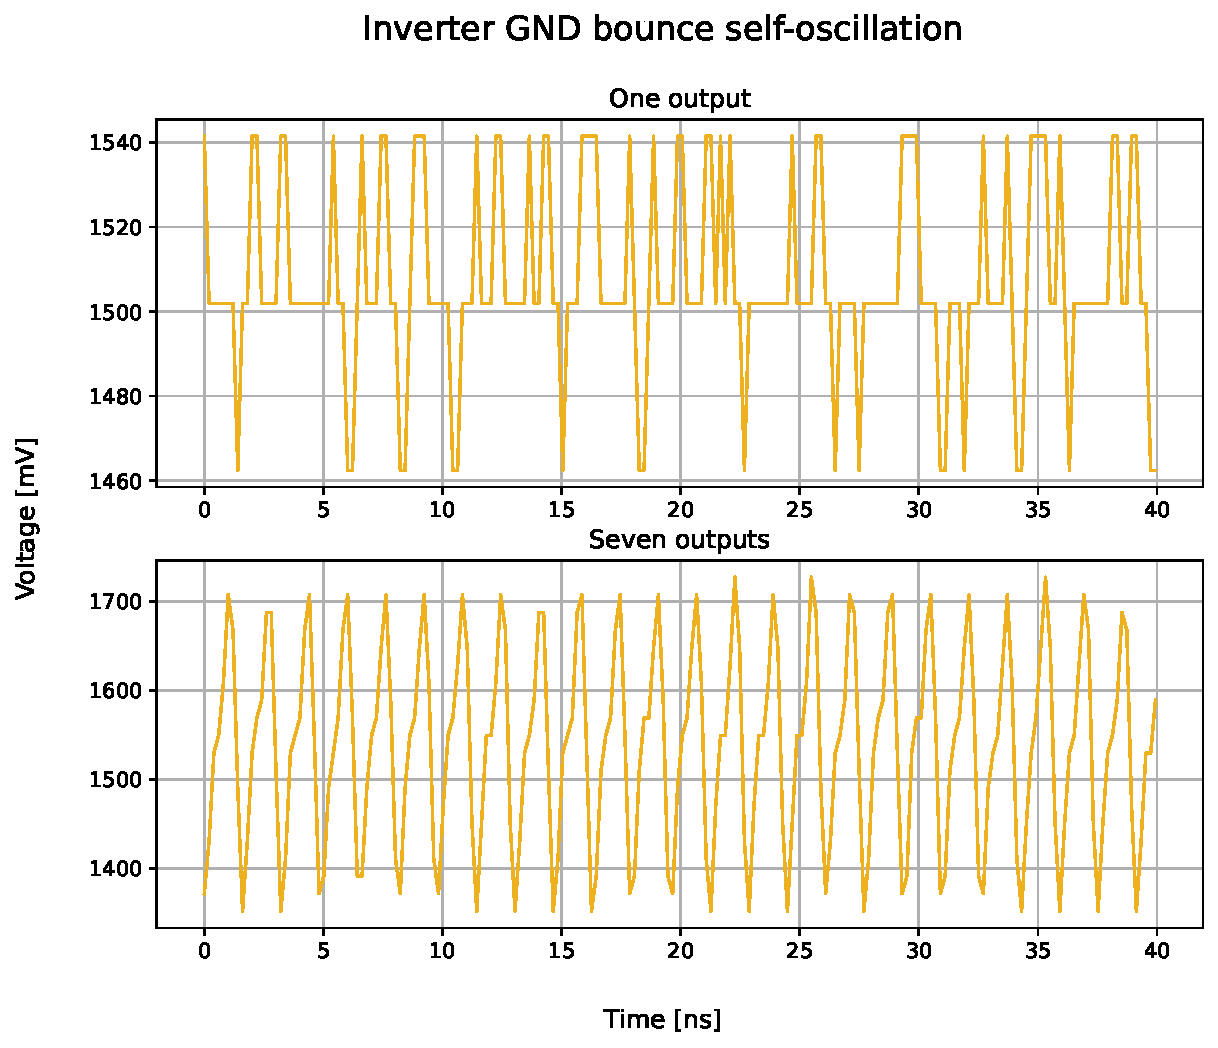
\includegraphics[width=0.8\textwidth]{osci.pdf}
    \caption{Measured oscillations of the inverter output with one and all outputs active.}
    \label{fig:inverter_oscillation}
\end{figure}

\end{document}
